\section{Implementation}
\label{sec:implementation}
In this section, we discuss the implementation of various parts the viscous democracy voting model. Firstly, we explain the construction and details of the social graph of Wikipedia editors. Next, we describe the different approaches to form the delegation rule. Lastly, we see the details of the local and global tally methods.

\subsection{Social Graph}
As described in Section~\ref{sec:user-contrib}, the \usercontrib dataset has comprehensive edit history for each user. We use edits from the \textit{User Talk Page} namespace to create an edge in the social graph. The nodes are limited to the users from the RfA dataset so that the size of the graph is not unnecessarily large. An edge exists between user $u$ and user $u$ if $u$ has edited $v$'s talk page. This provides an underlying directed social interaction graph. The properties of the network are show in Table~\ref{tab:social-graph}.

\begin{table}
    \centering
    \begin{tabular}{lr}
        \toprule
        \textbf{Property}& \textbf{Value} \\
        \midrule
        Number of Node & $12\,529$ \\
        Number of Edges & $1\,149,415$ \\
        Density & $0.00732$\\
        Largest connected component size &$10\,565$\\
        \bottomrule
    \end{tabular}
    \caption{Social Graph properties}
    \label{tab:social-graph}
\end{table}

We see that the size of the social graph is smaller than the total number of unique users. This is due to many user changing names or accounts being inactive. The graph is also fairly well connected with a single large connected component and all others are singleton components which correspond to temporary or one-time users. The graph is inherently directed and the successors and predecessors of a node can provide information on whom the node has contacted or who have contacted the node respectively. if we convert the graph into an undirected network the neighbours of a node $u$ are the union of the successors and predecessors. We will use this social graph as the basis of neighbours or contacts for voters in the viscous democracy model.

\subsection{Delegation Rule}
The most important part of the model is the delegation rule. In their work, Boldi et al.\ \cite{ViscousDemocracy} mention that delegation usually happens within the community and that once delegation occurs you can use the viscous democracy to evaluate the scores of each node in the graph. The difficulty is that when using this model to simulate an election we require a heuristic by which people delegate within their neighbourhood. Boldi et al.\ in their simulation of voting in a co-authorship network used the criteria that a voter would delegate to the person in their neighbourhood who has published more papers, if none exists then they would vote for themselves, choosing not to delegate themselves.

Therefore, in our simulation of Wikipedia RfA elections, we use the attributes of each voter to decide how the delegation would be carried out. We recorded the following information for each node\footnote{the terms node, voter and users can be used interchangeably} in the social graph:
\begin{enumerate}
    \item Start date of the account
    \item Total number of edits
    \item Ranking
\end{enumerate}
Each of these features results in a different delegation rule which are called \textbf{seniority}, \textbf{edit count} and \textbf{rank} respectively. Given a node $u$ we will define the neighbourhood of the node as $\mathcal{N}_u$. As mentioned previously the nodes in the neighbourhood depends on whether the graph is directed or undirected. The augmented neighbourhood is defined as appending the node $u$ to the neighbourhood denoted by ${\mathcal{N}_u}^\prime = \mathcal{N}_u \cup u$. We explain each rule and how it will be applied to the social graph.

\subsubsection{Seniority Rule}
This rule is based on the start date of each node. The delegation will be done to the node that has the most seniority, i.e., the earliest starting date. If the function $\startdate(v)$ returns the start date of node $v$ then the delegation function can be written as follows where $\seniority(\cdot)$ is the delegation rule based on seniority.
\[\seniority(u)  = \argmin_{v \in \mathcal{N}_u^\prime} \left( \startdate(v) \right).\]
This delegation rule is based on the heuristic that people who have been an editor in Wikipedia longer are better placed to make a decision on the administrative qualities of a candidate. 

\subsubsection{Edit Count Rule}
This heuristic is based on the fact that the users on Wikipedia who have more edits are usually more active in the community and are therefore the ones whose votes will be most influential in swaying other voters to support a candidate. Hence given a node $u$ we take the augmented neighbourhood $\mathcal{N}_u^{\prime}$ and then choose the node which has the highest number of total edits to delegate to. In this way, if there is no neighbour who has more edits than the node $u$ then, the user votes for herself. We define the function $\editcount(v)$ to return the total number of edits for user $v$ and $\edit$ as the delegation function based on edit count. We have 
\[\edit(u)  = \argmax_{v \in \mathcal{N}_u^\prime} \left(\editcount(v) \right).\]

\subsubsection{Rank Rule}
If there exists a hierarchy in the social network then we can use that as a heuristic upon which to delegate votes. It works the same way that the other delegation rules have been defined. Given a node we delegate to the neighbour who has the highest rank, if not then the node votes for herself. This style of voting is particularly useful in societies where is there is some organizational structure. However, there is no such defined structural hierarchy amongst Wikipedia editors. Moreover, the administrators themselves are no different than editors with access to tools to help with their roles. Therefore, the first requirement is to find a hierarchy in the directed social graph.

There is already existing work in finding hierarchies in directed networks using concepts such as the concept of \textit{agony} \cite{Tatti2016,gupte2011finding}. If each node in a directed graph $G = (V,E)$ is given a ranking, formally defined as $r:V\rightarrow \mathbb{N}$ then any edge $u\rightarrow v$ causes agony if $r(u)\geq r(v)$ and is equal to difference plus one, i.e., $r(u)-r(v)+1$. The agony of the whole network $G$ with respect to the ranking $r$ is the summation of the agony caused by every edge $e \in E$. The concept of agony is based on the principle that people higher up in a social hierarchy do not prefer to interact with people lower down in the hierarchy. This is the reason why edges $u\rightarrow v$ where $r(u)<r(v)$ causes no agony. Gupte et al.\ \cite{gupte2011finding} go on to show that the measure of agony of a network corresponds to how close a network is to being a Directed Acyclic Graph (DAG). As DAGs have perfect hierarchies this means that they have a corresponding agony of $0$. Therefore, the ranking $r$ is the proposed hierarchy of the network. Gupte et al.\ provide a method of uncovering this hierarchy in a network by solving the problem of finding the ranking $r$ that minimizes the agony of a network. Tatti \cite{Tatti2016} provides an algorithm that can solve this problem in polynomial time by solving the dual problem of finding the maximum Eulerian subgraph. We use the algorithm and code of Tatti\footnote{http://users.ics.aalto.fi/ntatti/agony.zip} to find the ranking for the social graph of Wikipedia editors. 

This method of finding the hierarchy penalizes edges from high rank to low rank. This means we must understand the context of a link in the case of the social graph. In the social graph, an edge $u \rightarrow v$ indicates that user $u$ has written in the talk page of $v$. Therefore, we must ask ourselves if agony occurs when lower ranked users write on higher ranked user pages or if it occurs in the opposite direction. To not restrict ourselves to one approach we computed the rank for both possibilities. In the regular case, this means that agony is caused when high rank users write on low rank user talk pages. The other case is the reversed social graph, where an edge $u \rightarrow v$ means that $v$ has written in talk page of $u$, and here agony occurs when a lower ranked member writes in a higher ranked user's talk page. We will call the ranks derived from this reversed social graph as \textit{reversed ranks}. 

We see the distribution of the ranks in Figure~\ref{fig:rank} \& \ref{fig:reversed-rank}. The number of levels are different with regular ranking having $8$ and reversed ranking having $9$ levels of hierarchy. In both distributions, we see that the highest level of hierarchy has only around 100 users. This again points to the fact that there exists a small core of influential users in the network based only on their interactions. We can now use the rank that each node had to create two distinct delegation rules.

Given a node $u$ we take the augmented neighbourhood $\mathcal{N}_u$ and then choose the node which has the largest rank or reversed rank from the set. The functions $\rank(v)$ and $\revrank(v)$ provide the rank and reversed rank of the node $v$ respectively and the delegation functions $\rankdelegate(u)$ and $\revrankdelegate(u)$ for rank and reversed rank respectively are defined as 
\[\rankdelegate(u)  = \argmax_{v \in \mathcal{N}_u^\prime} \left(\rank(v) \right).\]
\[\revrankdelegate(u)  = \argmax_{v \in \mathcal{N}_u^\prime} \left(\revrank(v) \right).\]

\begin{figure}[!ht]
    \centering
    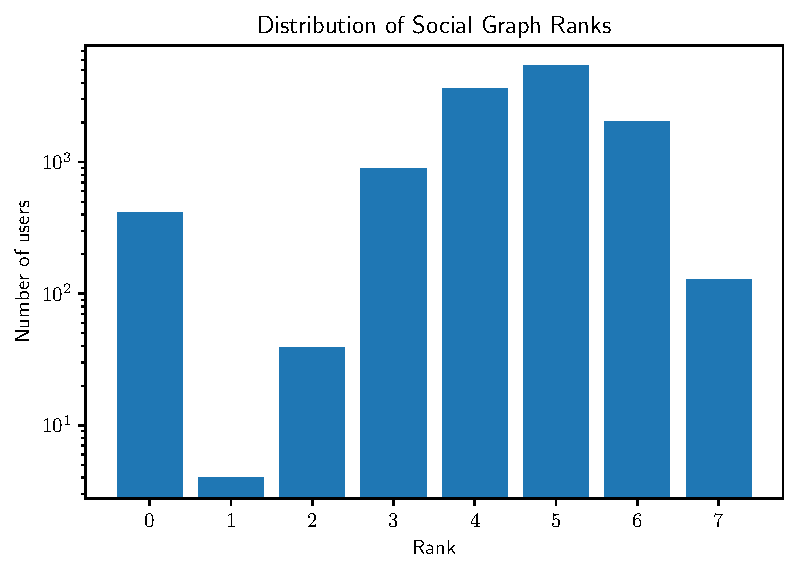
\includegraphics[width=\linewidth]{images/Rank dist.pdf}
    \caption{Rank Distribution in Social graph}
    \label{fig:rank}
\end{figure}
\begin{figure}[!ht]
    \centering
    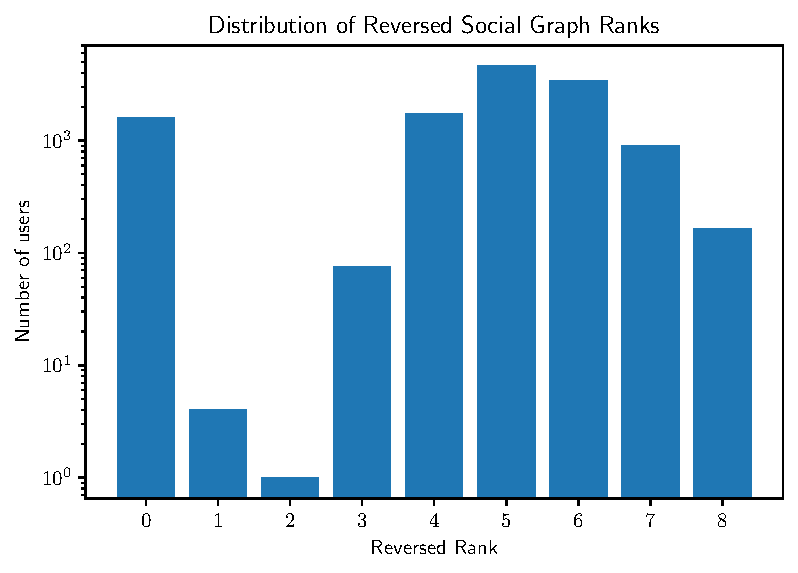
\includegraphics[width=\linewidth]{images/Reversed Rank dist.pdf}
    \caption{Rank Distribution in Reversed Social graph}
    \label{fig:reversed-rank}
\end{figure}

\subsection{Tally Schemes}
Now, after implementing the social graph of Wikipedia users and simulating the delegation using any one of the delegation rules, we have a delegation graph. From the delegation graph we can get the node scores by computing Katz's centrality measure with a given value of $\alpha$. These node scores defined as a function $s:V\rightarrow \mathbb{R}$ can be used to predict elections as discussed in Section~\ref{sec:tally}. In both tally approaches we want to select top $k$ users and then predict an election by tallying their votes. This can be either in a global context or a local context. We now describe these two approaches.
\subsubsection{Global Tally}
In the global context, we take all the nodes of the social graph and then choose $k$ users with the largest scores obtained from the previous steps. Then, we go through each particular RfA and then only take the votes corresponding to the chosen $k$ users and then tally their votes. We then predict the election is successful is there are more support votes, unsuccessful if more oppose than support and a neutral outcome otherwise. This method aims to find a constant core set of influential users obtained from the viscous democracy model. As most users do not vote in every election, we would need a large set of users to have a good predictive accuracy across all the elections in the dataset. As $k$ approaches $N$, where $N= |V|$ of the social graph, we take all users and their votes in each election to predict the results. 
\subsubsection{Local Tally}
The local context of tallying is when we take an RfA election and then of all the users who voted we choose the $k$ with the largest scores and only tally their votes. We consider a support vote as $+1$, oppose vote as $-1$ and a neutral vote as $0$. Then the tally of $k$ votes would be the sum of all the $k$ votes. We predict a successful elections if the tally is positive, unsuccessful if the tally is negative and neutral if the tally is exactly 0. It is evident that in this method that the top $k$ users are not unique and change based on the RfA being predicted. This also means that the size of $k$ could be smaller and might lead to similar and possibly better predictive power compared to the global context.

\subsection{Hyperparameters}
The viscous democracy model has many parameters and hyperparameters that can be varied. These occur in different stages of the model and affect the final predictive accuracy of the model. In this subsection we will list all these hyperparameters and their possible values.

\begin{itemize}
    \item $\boldsymbol{\alpha}$ : the delegation factor, $\alpha\in (0,1)$
    \item $\mathbf{k}$ : number of users to consider using node scores, $k \in \mathbb{N}$
    \item \textbf{Delegation Rule}: Seniority, Edit Count, Rank or Reversed Rank 
    \item \textbf{Tally Scheme}: Local or Global
    % \item \textbf{Social Graph Type}: Directed or Undirected
\end{itemize}
We see that there are many possible combinations of parameters and hyperparameters to arrive at a model. In the following section we will present the results of the proposed model. 